\documentclass[12pt, unicode]{beamer}
\usetheme{Warsaw}
\usepackage{luatexja}
\usepackage{color}
\usepackage{listings}
\lstloadlanguages{Ruby}
\lstset{%
  language=Ruby,
  basicstyle=\ttfamily\color{black},
  commentstyle = \ttfamily\color{red},
  keywordstyle=\ttfamily\color{blue},
  stringstyle=\color{orange}
}
\setbeamertemplate{navigation symbols}{}

\title{Fluentdの開発支援の話}
\subtitle{FluentdのWindows版の機能に関わる開発支援の裏話}
\author{Hiroshi Hatake}
\institute[Clear Code Inc.]{株式会社クリアコード}
\date[2016/07/30]{Fluentd meetup in Matsue}

\begin{document}

\frame{\maketitle}

\begin{frame}{自己紹介}
  \begin{itemize}
  \item Hiroshi Hatake \newline 
\includegraphics[clip,width=2cm]{images/yuudachi.png}
    \begin{itemize}
    \item Twitter: @cosmo\_\_
    \item GitHub: @cosmo0920
    \end{itemize}
  \item 株式会社クリアコード
  \item OSSサポート(開発・導入支援・時間制サポート etc.)をしています。\footnote[frame]{https://www.clear-code.com/services/floss/development.html}
  \end{itemize}
\end{frame}

\section[]{はじめに}
\begin{frame}{}
 \tableofcontents
\end{frame}

\section[]{Fluentdの開発支援の話}
\begin{frame}{Fluentdの開発支援の話}
  \begin{block}{{開発支援でやってきた内容}}
    \begin{itemize}
    \item Fluentd 0.12.16のsecret parameterが入った前後から開発支援をしています
    \item メモリダンプの機能
    \item Parser/Formatterのテストドライバ
    \item built-inのプラグインのv0.14のAPIへの移行
    \item AppVeyorの導入のお手伝い
    \item \only<1>{メンテナンスが活発でないgemを引き取ってメンテナンス}\only<2>{\alert{メンテナンスが活発でないgemを引き取ってメンテナンス}}
    \item プラグインへ各種PR etc.
    \end{itemize}
  \end{block}
\end{frame}

\begin{frame}{Fluentdの開発支援の話}
  \Large{Fluentd v0.14の開発支援をしていく中で、FluentdのWindows向けの機能で依存しているgemのメンテナンスを引き取った話をします。}
\end{frame}

\section[]{Fluentd v0.14の新機能のおさらい}
\begin{frame}{Fluentd v0.14の新機能のおさらい}
  \Large{
    \begin{itemize}
    \item \only<1>{Windowsサポート}\only<2->{\alert{Windowsサポート}}
    \item 高精度な時刻サポート
    \item 新しいプラグインAPI
    \item routerの使用の強制 \footnote[frame]{Engine.emitがバグ扱いになりました}
    \end{itemize}
  }
\end{frame}

\begin{frame}{FluentdのWindowsサポート}
  \Large{
    \only<1>{つまり、Fluentd v0.14の開発ではWindowsも考慮した開発が必要。}
    \only<2>{つまり、Fluentd v0.14の開発では\alert{Windowsも考慮した開発が必要。}}
  }
\end{frame}

% Set font size for lstlisting.
\newcommand\Small{\fontsize{9}{9.5}\selectfont}
\section[]{FluentdのWindowsサポート}
\begin{frame}[fragile]{FluentdのWindows版で増えている依存関係(抜粋)}
\begin{lstlisting}[language=Ruby,basicstyle=\ttfamily\Small]
if /mswin|mingw/ =~ RUBY_PLATFORM
  gem.add_runtime_dependency("win32-service", ["~> 0.8.3"])
  gem.add_runtime_dependency("win32-ipc", ["~> 0.6.1"])
  gem.add_runtime_dependency("win32-event", ["~> 0.6.1"])
  gem.add_runtime_dependency("windows-pr", ["~> 1.2.5"])
end
  \end{lstlisting}
\end{frame}

\begin{frame}{Windows版で増えている依存関係}
  \Large{
    \begin{itemize}
    \item win32-service
    \item win32-ipc
    \item win32-event
    \item windows-pr
      \begin{itemize}
      \item windows-api
      \item win32-api
      \end{itemize}
    \end{itemize}
  }
\end{frame}

\begin{frame}{今回話す話す内容のgemとFluentdの関係図}
  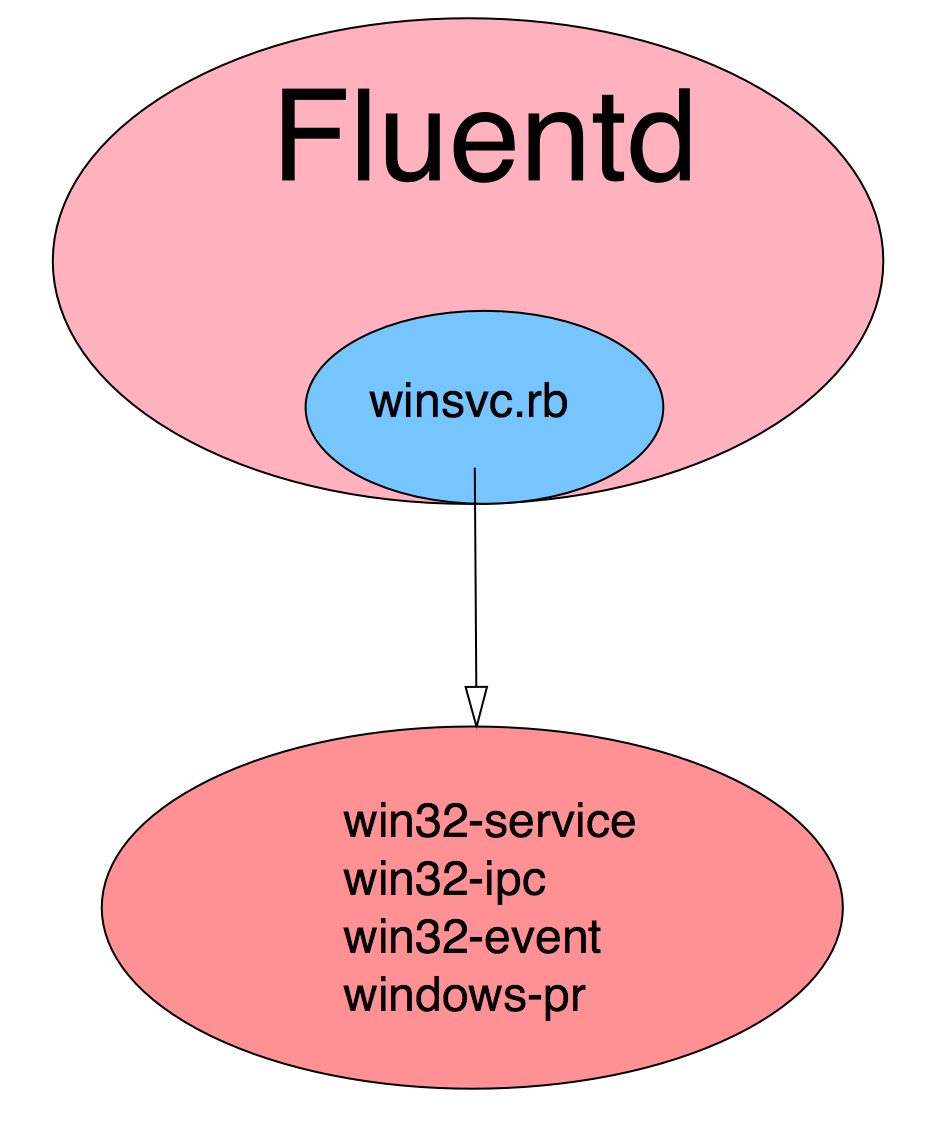
\includegraphics[clip,width=6cm]{images/Fluentd_windows_version_dependent_gems.png}\newline
  Windowsサービスに関わる箇所(winsvc)が依存しています。
\end{frame}

\begin{frame}{今回話す話す内容に関わるgemたち}
   \Large{
    \begin{itemize}
    \item windows-pr
    \item windows-api
    \item \only<1>{win32-api}\only<2>{win32-api \alert{C拡張を含むgem}}
    \end{itemize}
  }
\end{frame}

\begin{frame}{C拡張とは?}
  \uncover<1-> {
    \begin{block}{C拡張で何かできるの?}
      RubyにはC extensionというCによりRubyを拡張できる機能があります。\newline
      これにより、Cのライブラリの機能をRubyに取り込むことができます。
    \end{block}
  }
  \uncover<2-> {代表例:}
  \begin{itemize}
  \item <3-> WindowsのCOMの機能をバインドしたWin32OLE
  \item <4-> GroongaのCライブラリをバインドしたRroonga
  \item <5-> GTK+のライブラリをバインドしたRuby-GNOME2
  \end{itemize}
\end{frame}

\begin{frame}{C拡張とは?}
  \begin{block}{C拡張を含むgemの注意点}
    \begin{itemize}
    \item gemのユーザーは依存しているライブラリをシステムにインストールする必要があります
      \begin{itemize}
      \item \only<1>{実はdllやdylibだけでもRubyのC拡張から機能が呼べることができれば使う分には大丈夫です。}
        \only<2>{\alert{実はdllやdylibだけでもRubyのC拡張から機能が呼べることができれば使う分には大丈夫です。}}
      \end{itemize}
    \item gemのユーザーはCのソースをビルドするための開発環境をシステムにインストールする必要があります
    \end{itemize}
  \end{block}
\end{frame}

\section[]{WindowsでのRubyのエコシステム}
\begin{frame}{WindowsでのRubyのエコシステム}
  \begin{block}{fat gemとは}
    \begin{itemize}
    \item {\bf fat gem} というgemの中にRubyのC拡張のバイナリをパッケージングできるしくみがあります。
    \item Fluentdでも使っているcool.io\footnote[frame]{https://github.com/tarcieri/cool.io}でもこの仕組みを使用しています。
    \end{itemize}
  \end{block}
\end{frame}

\begin{frame}{RubyのC拡張のバイナリをgemにパッケージング}
  \begin{block}{利点・欠点}
    \begin{itemize}
    \item 利点
      \begin{itemize}
        \item C拡張を予め入れておくことで、WindowsでRubyを使うユーザーがC拡張をビルドしなくてもよくなります
      \end{itemize}
    \item 欠点
      \begin{itemize}
        \item 新しいRubyが出たらそれ用のgemをリリースしなければならない
        \item 開発者がパッケージングする手間が増える
        \item クロスコンパイルするのに一手間
      \end{itemize}
    \end{itemize}
  \end{block}
\end{frame}

\begin{frame}{RubyのC拡張のバイナリをgemにパッケージング}
  \begin{block}{それでもfat gemを提供する理由}
    \begin{itemize}
    \item ユーザーからするとfat gemが提供されていた方が嬉しい
    \item Windowsユーザーはあまり開発環境を構築していない
    \end{itemize}
  \end{block}
\end{frame}

\section[]{win32-api gemのサポート}
\begin{frame}{win32-api gem}
  \begin{block}{win32-apiとは}
    元はdjberg96氏\footnote[frame]{https://github.com/djberg96}作。\newline
    Win32APIをRubyから呼び出せるラッパー。\newline
    Ruby本体のAPIにはないコールバックサポートがあります。
    {\bf $\#include <windows.h>$ }\# WIN32APIのおまじない
  \end{block}
\end{frame}

\begin{frame}{win32-apiのRuby 2.3サポート}
  \large{
    \begin{block}{Ruby 2.3がサポートされていなかったのでIssueを上げました}
      Support precompiled binaries for Ruby 2.3: \newline
      https://github.com/djberg96/win32-api/issues/16
    \end{block}
  }
\end{frame}

\begin{frame}{win32-apiのRuby 2.3サポート}
  \Large{
    \begin{block}{}
      @djberg98 ``@cosmo0920 I don't suppose you would be interested in taking over this project, would you?''\footnote[frame]{https://github.com/djberg96/win32-api/issues/16\#issuecomment-212021651}
    \end{block}
  }
\end{frame}

\begin{frame}{win32-apiのRuby 2.3サポート}
  \Large \only<1>{つまりどういうこと?}\only<2>{真意がよくわからないので聞いてみましょう}
\end{frame}

\begin{frame}{win32-apiのRuby 2.3サポート}
  \Large {
    \begin{block}{}
      \begin{itemize}
      \item \uncover<1->{@cosmo0920(me) ``What do you want to do for me?
      Just building universal gem? Or, entirely taking over this project?''}
      \item \uncover<2->{@djberg96 ``@cosmo0920 Completely taking over project.'' }
      \end{itemize}
    \end{block}
  }
\end{frame}

\begin{frame}{win32-apiのRuby 2.3サポート}
  \Large {
    \center {
      \uncover<1->{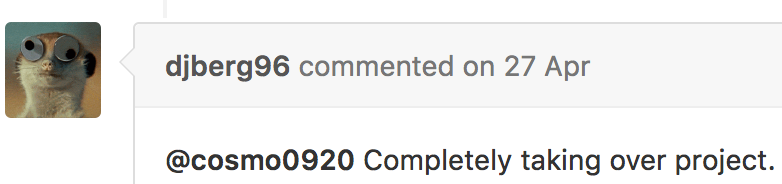
\includegraphics[clip,width=9.5cm]{images/reply_djberg96_in_win32-api_issue}}\newline
      \only<2>{訳:完全に引き継いでください。}
      \only<3>{\alert{訳:完全に引き継いでください。}}
    }
  }
\end{frame}

\begin{frame}{win32-apiのRuby 2.3サポート}
  \begin{block}{実はメンテナを探していた}
\uncover<1->= Maintainer Wanted!
Since I no longer use this project, I would like to turn it over to
someone who has the skill, time and desire to keep it going.\footnote[frame]{https://github.com/cosmo0920/win32-api/blob/eef0b35dd095f43cac0d48824a782ecbb31a25d6/README\#L118}\newline
\uncover<2->{訳: メンテナ求む! このプロジェクトはもう使っていないので、技術があり、時間と続けていく心意気のある誰かに譲りたい。}
  \end{block}
\end{frame}

\begin{frame}{win32-apiのRuby 2.3サポート}
  \Large {
    \uncover<1->{win32-apiプロジェクトのmasterを引き継ぎました。}\newline
    \small{\uncover<2->{windows-api, windows-prプロジェクトのmasterも合わせて引き継ぎました。}}
  }
\end{frame}
\begin{frame}{win32-apiのRuby 2.3サポート}
  Ruby 2.3に対応させる\footnote[frame]{https://github.com/cosmo0920/win32-api/pull/18}作業と、AppVeyorの導入\footnote[frame]{https://github.com/cosmo0920/win32-api/pull/20}の作業を行いました。
  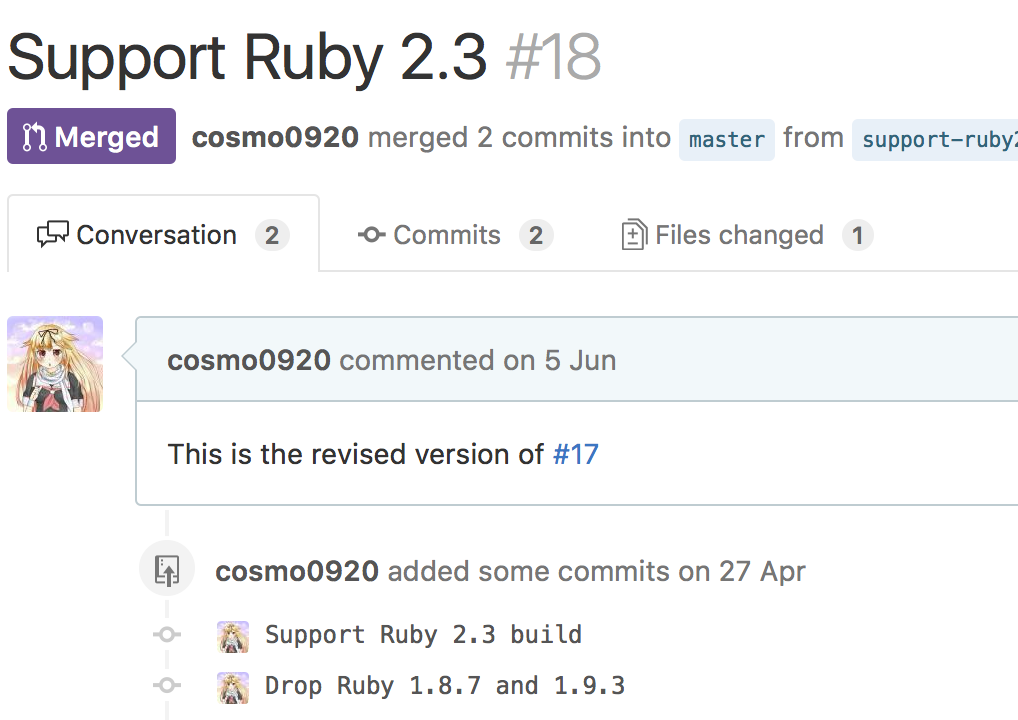
\includegraphics[clip,width=4cm]{images/support_ruby23_win32-api}
  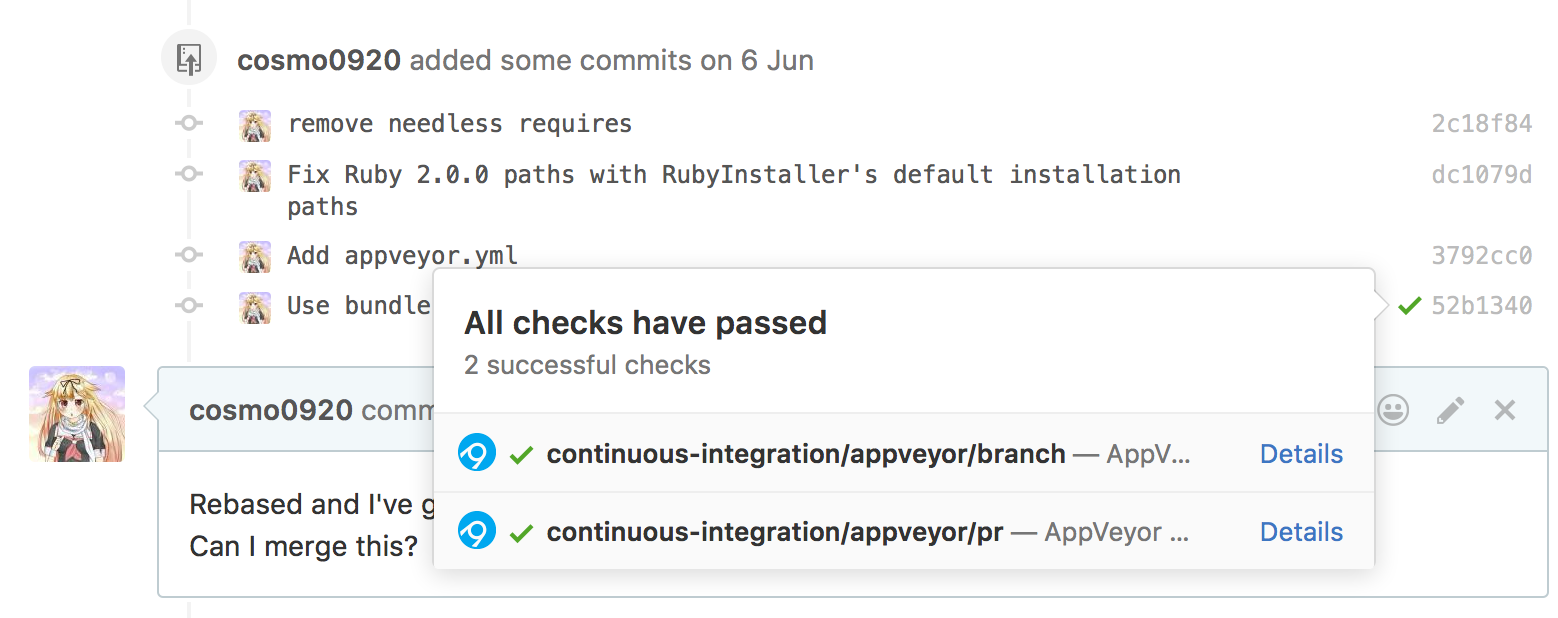
\includegraphics[clip,width=7cm]{images/support_appveyor_win32-api}
\end{frame}
\begin{frame}{win32-apiのRuby 2.3サポート}
  \Large {
   \center {1.6.0としてRuby 2.3のサポートと、Ruby 1.8.7と1.9.0のサポートを切ったバージョン1.6.0をリリース済みです。\footnote[frame]{https://rubygems.org/gems/win32-api/versions/1.6.0-universal-mingw32}}
  }
\end{frame}

\begin{frame}{windows-api gemのサポート}
  \begin{block}{windows-api gem}
    AppVeyorの導入をしました。\footnote[frame]{https://github.com/cosmo0920/windows-api/pull/6}
  \end{block}
  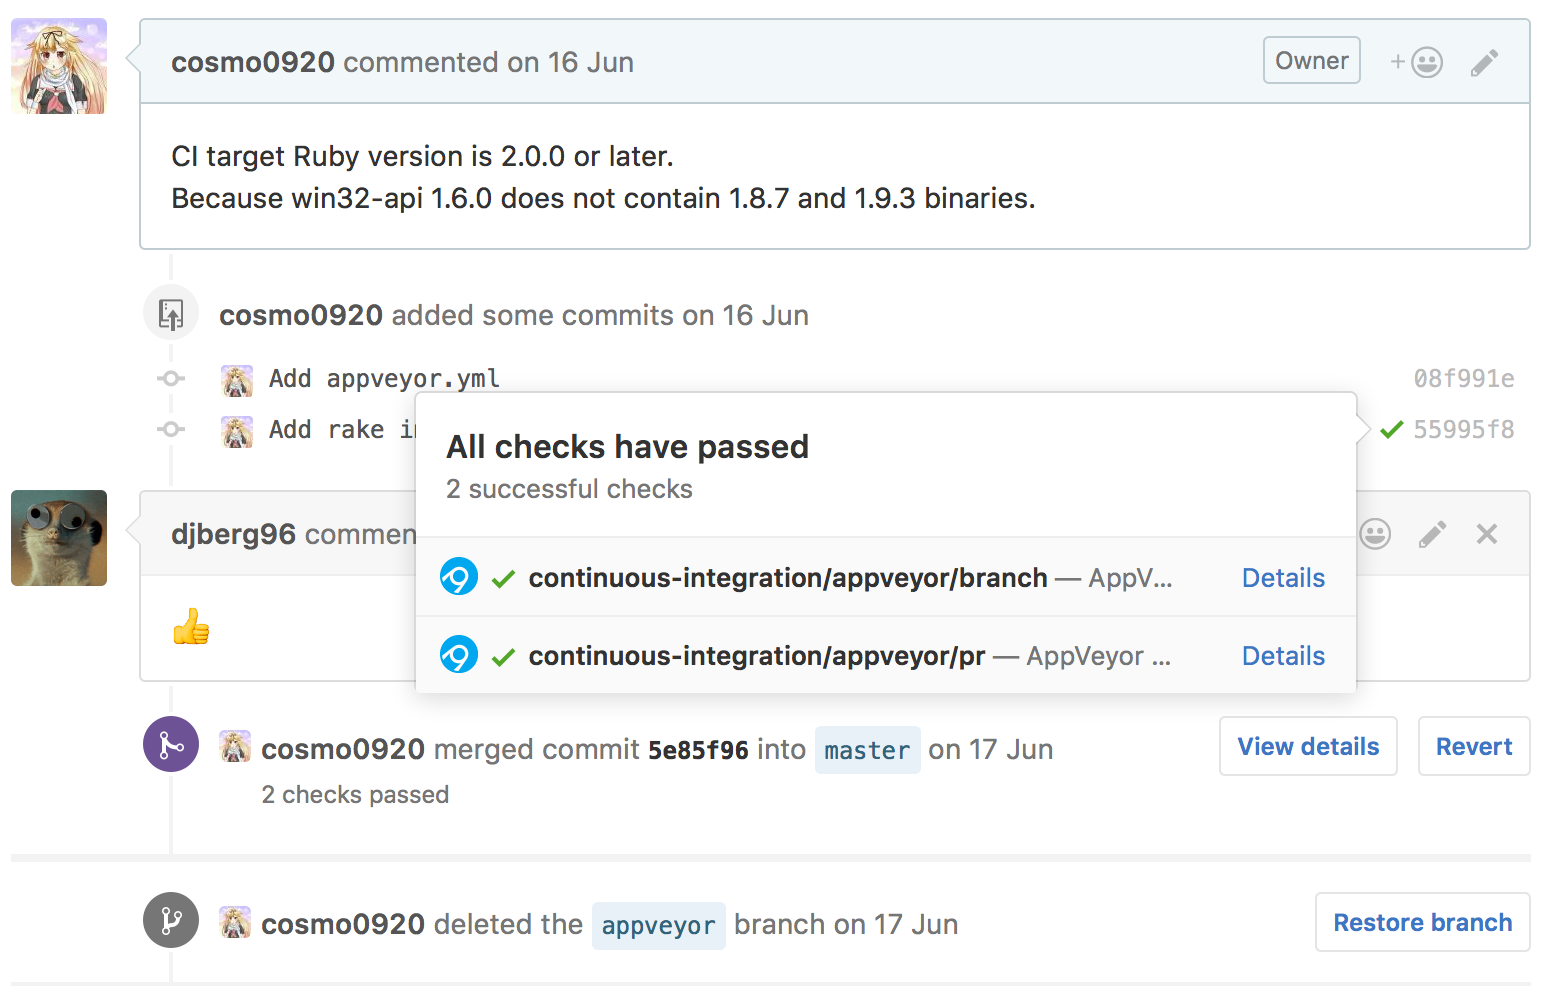
\includegraphics[clip,width=9.5cm]{images/support_appveyor_windows-api_gem.png}
\end{frame}

\section[]{windows-pr gemのFluentdに関わるIssueの解決}
\begin{frame}{windows-pr gem}
  \begin{block}{windows-pr gemのサポート}
メンテナンスを引き継いでからすぐにIssueを解決することとなりました。\footnote[frame]{https://github.com/cosmo0920/windows-pr/issues/13}\newline
対応するFluentd側のIssueは https://github.com/fluent/fluentd/issues/920
  \end{block}
\end{frame}

\begin{frame}{windows-pr gemのサポート}
  \begin{block}{in\_tailがWindows上で問題を起こしていた}
    in\_tailで監視しているファイルが削除されると、\newline
    $undefined method `pe=' for \#<Fluent::TailInput::TailWatcher::NullIOHandler:::0x0000000XXXXXXXX>"`$
    というエラーが起きていました。
  \end{block}
\end{frame}

\begin{frame}{windows-pr gemのサポート}
  \begin{block}{何が起きていたのか}
    \begin{itemize}
    \item INVALID\_HANDLE\_VALUEが32bitと64bitでは異なる定数として扱わなければなりません。しかし、0xFFFFFFFFがハードコートされてしまっていました。
    \item 64bit環境ではINVALID\_HANDLE\_VALUEが0xFFFFFFFFFFFFFFFFとなるように修正しました。\footnote[frame]{https://github.com/cosmo0920/windows-pr/pull/15} \footnote[frame]{ただし、この修正はCRubyに対しては有効で、JRubyに対してはバグを含んでいます。}
    \end{itemize}
  \end{block}
\end{frame}

\begin{frame}{windows-pr gemのサポート}
  無事、治ったとのこと。
  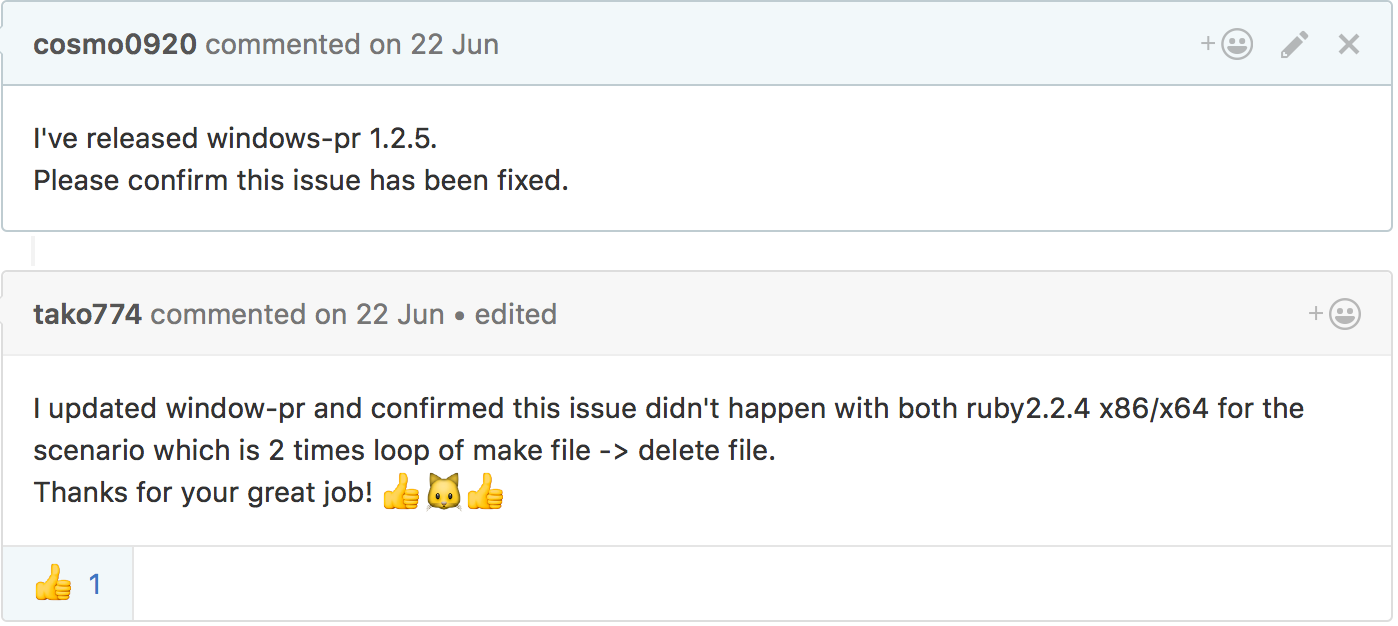
\includegraphics[clip,width=11cm]{images/fixed_in_tail_invalid_handle_in_windows.png}
\end{frame}

\begin{frame}{windows-pr gemのサポート}
  \Large {
   \center {INVALID\_FILE\_HANLDEの64bit Windows環境での定数の不具合を修正したバージョン1.2.5をリリース済みです。\footnote[frame]{https://rubygems.org/gems/windows-pr/versions/1.2.5}}
  }
\end{frame}

\section[]{まとめ}
\begin{frame}{まとめ}
  \begin{block}{}
    FluentdのWindows版の機能で依存しているgemのメンテナンスを引き取った話をしました。\newline
    その際に、単に引き取るだけでなく、よりメンテナンスがしやすい方向にしていく変更を入れました。\newline
    WindowsでRubyを使う際には、C拡張やWindowsに関わるRubyやgemの問題に対応しているメンテナの存在を思い出してあげてください。
  \end{block}
\end{frame}
\end{document}
